\scanpage{78}
\uline{Complexe de \unsure{cotie} des groupes de \unsure{t.m.}.}

1. Soit $G=D(M)$, $M$ un réseau sur $S$ = \unsure{grpe|groupe} ct tordu sur $S$.

Considérons la résolution plate canonique en deux crans
\[
\tag{1.1}
\diagram{\begin{tikzcd}0\arrow[r]&R\arrow[r,"v"]&\mathbb Z[M]\arrow[r,"u"]&M\arrow[r]&0\end{tikzcd}},
\]
\unsure{où} $R=\operatorname{Ker}u$, $u([m])=m$. On en déduit, par passage aux duals, une suite exacte
\[
\tag{1.2}
\diagram{\begin{tikzcd}
0\arrow[r]&G\arrow[r,no head]&T\arrow[r,no head]\arrow[d,equal]&T'\arrow[r,no head]\arrow[d,equal]&0\\
&&\mathbb G_m^M&D(R)&
\end{tikzcd}}
\]
résolvant $G$ par des tores. (\unsure{évt} de dim. relative infinie\dots).

Le triangle de transitivité de \unsure{Mazur-Roberts} donne un isomorphisme
\deleted{$\unsure{\ell_G|L_G}$}
\[
\ell_\bullet^G\simeq
\left[\diagram{\begin{tikzcd}\omega_{T'}\arrow[r,no head]&\omega_T\end{tikzcd}}\right]
\simeq\left[\diagram{\begin{tikzcd}R\otimes_{\mathbb Z}\mathcal O_S\arrow[r]&\mathbb Z[M]\otimes_{\mathbb Z}\unsure{\mathcal O_S}\end{tikzcd}}\right.
\]
i.e.
\[
\tag{1.3}
\boxed{\ell_\bullet^G\simeq\underline M\overset{\mathbf L}{\otimes}_{\mathbb Z}\underline{\mathcal O}_S}
\]
\figure{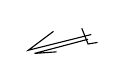
\begin{tikzpicture}[x=.4cm,y=.4cm]
\draw (2,.5)--(0,0)--(.8,.6);\draw (1.9,.35)--(.2,-.1)--(.9,-.05);
\draw (1.7,.7)--(1.9,.2)--(2.2,.25);
\end{tikzpicture}}
Si \deleted{\unsure{on}} $\mathcal O_S$ est \unsure{une} $\Lambda$-Algèbre (p.ex. $\Lambda=\mathbb Q$, ou $\Lambda=\mathbb Z/n\mathbb Z$)

\deleted{$n\mathcal O_S=0$, i.e. $\mathcal O_S$ une $\mathbb Z/n\mathbb Z$-Algèbre,}

on peut écrire aussi
\[
\tag{1.4}
\boxed{\ell_\bullet^G\simeq
\bigl(M\overset{\mathbf L}{\otimes}_{\mathbb Z}\Lambda\deleted{\unsure{\mathbb Z/n\mathbb Z}}\bigr)
\overset{\mathbf L}{\otimes}_{\Lambda\deleted{\unsure{\mathbb Z/n\mathbb Z}}}\mathcal O_S}
\]
et si
\mspage{77}
